\documentclass{aa}

\usepackage{graphicx}

\usepackage[varg]{txfonts}
\usepackage{units}
\usepackage{mathtools}
\usepackage{color}
\usepackage{natbib,twoopt}
\usepackage{siunitx}
\usepackage{hyperref} %% to avoid \citeads line fills
\bibpunct{(}{)}{;}{a}{}{,}             %% natbib format for A&A and ApJ
\makeatletter
  \newcommandtwoopt{\citeads}[3][][]{\href{http://adsabs.harvard.edu/abs/#3}%
    {\def\hyper@linkstart##1##2{}%
     \let\hyper@linkend\@empty\citealp[#1][#2]{#3}}}
  \newcommandtwoopt{\citepads}[3][][]{\href{http://adsabs.harvard.edu/abs/#3}%
    {\def\hyper@linkstart##1##2{}%
     \let\hyper@linkend\@empty\citep[#1][#2]{#3}}}
  \newcommandtwoopt{\citetads}[3][][]{\href{http://adsabs.harvard.edu/abs/#3}%
    {\def\hyper@linkstart##1##2{}%
     \let\hyper@linkend\@empty\citet[#1][#2]{#3}}}
  \newcommandtwoopt{\citeyearads}[3][][]%
    {\href{http://adsabs.harvard.edu/abs/#3}
    {\def\hyper@linkstart##1##2{}%
     \let\hyper@linkend\@empty\citeyear[#1][#2]{#3}}}
  \renewcommand*\aa@pageof{, page \thepage{} of \pageref*{LastPage}}
\makeatother
\hypersetup{pdfpagemode = {UseNone},
            pdftitle = {Theory of dics photoevaporation},
            pdfcreator = {\LaTeX},
            pdfproducer = {pdfeTeX-0.\the\pdftexversion\pdftexrevision},
            pdfauthor = {Giovanni Picogna, Barbara Ercolano, Catherine Espaillat},
            pdfsubject = {},
            pdfview = {FitH},
            pdfstartview = {FitH},
            colorlinks = {true},
            linkcolor = [rgb]{0,0.35,0.7},
            citecolor = [rgb]{0,0.35,0.7},
            filecolor = [rgb]{0.61,0,0},
            urlcolor = [rgb]{0,0.35,0.7},
           }

\usepackage{afterpage}
\usepackage{silence}
\WarningFilter{latex}{Text page}

\newcommand{\new}[1]{{\bf \color{black} #1}}
\newcommand{\todo}[1]{{\bf \color{red} #1}}

\begin{document}

    \title{Influence of stellar properties on disc photoevaporation}

    \author{
        Giovanni Picogna \inst{1} \href{https://orcid.org/0000-0003-3754-1639}{
\includegraphics[scale=0.04]{orcid}} \and
        Ercolano Barbara \inst{1,2}
        \href{https://orcid.org/0000-0001-7868-2740}{
\includegraphics[scale=0.04]{orcid}}
        \and
        Catherine Espaillat \inst{3}
        \href{https://orcid.org/0000-0001-9227-5949}{
\includegraphics[scale=0.04]{orcid}}
    }

    \institute{
        Universit\"{a}ts-Sternwarte, Ludwig-Maximilians-Universit\"{a}t M\"{u}nchen,
        Scheinerstr. 1, D-81679 M\"{u}nchen, Germany\\
        \email{picogna@usm.lmu.de, ercolano@usm.lmu.de}
        \and
        Excellence Cluster Origins, Boltzmannstrasse 2, D-85748 Garching bei M\"{u}nchen, Germany
        \and
        Department of Astronomy \& Institute for Astrophysical Research, Boston University, 725 Commonwealth Avenue, Boston, MA 02215, USA\\
        \email{cce@bu.edu}
    }

    \date{Received \today / Accepted \today}

    \abstract{}

    \keywords{accretion, accretion discs --
    protoplanetary discs --
    circumstellar matter --
    stars: pre-main-sequence --
    X-rays: stars.
    }

    \maketitle

%-------------------------------------------------------------------
\section{Introduction}
%-------------------------------------------------------------------

Our understanding of the physical processes driving the evolution of protoplanetary discs and ultimately the formation of planets is based on the observational evidence of disc lifetimes.

Strom et al. (1989) found that accretion discs are ubiqiutous around young stellar objects ($\sim 1$ Myr). The initial disc fraction is almost independent of stellar mass (from $0.1$ up to $10 M_\odot$) and stellar environment (Lada et al. 2000; Bouy et al. 2006).
After 10 Myr the picture changes completely since $> 90\%$ of stars show no emission within 1 au (Mamajek et al. 2004), and emission from small grains is found only in a few percent of discs (Liu et al. 2004; Carpenter et al. 2005; Silverstone et al. 2006).
This set an upper limit to the disc dispersal process within $10$ to $20$ Myr (Hernandez et al. 2007; Fedele et al. 2010; Ribas et al. 2014). Moreover, fitting the fraction of discs with dust emission at different wavelengths \citetads{2014A&A...561A..54R} found an e-folding time of $\sim2-3$ Myr at $3-12\, \mu m$ and $\sim4-6$ Myr at $22-24\, \mu m$, hinting at a inside-out dispersal of proto-planetary discs or to a second generation dust production.
The dust disc lifetime as a function of stellar mass is less well characterized but the dispersal timescale appears to be up to two times faster for high mass stars ($\geq 2 M_\odot$, Ribas et al. 2015).
The mass accretion onto the central star has also been studied extensively, though its evolution is less well constrained. Neverthless, it has been shown that the characteristic timescale of disc accretion is shorter than that of dust disc dispersal (Jayawardhana et al. 2006, Fedele et al. 2010), and the accretion rate falls off as a function of time with a power law (e.g., Manara et al. 2012; Antoniucci et al. 2014; Hartmann et al. 2016).

The main physical process driving disc dispersal is still largely unconstrained, and it might change during the disc evolution and at different locations in the disc. A large body of evidence is pointing at magneto-thermal disc winds as the main mechanism responsible for angular momentum transfer and mass-loss (Bai et al. 2015). From a theoretical stand-point there is a push to obtain better models that can be linked to observables in order to test their validity.

In the first paper of this series \citepads{2019MNRAS.487..691P} showed the dependance of the mass-loss rate due to thermal winds generated by the XEUV heating from the central star on the stellar X-ray luminosity. In this following work we focus on the stellar mass dependance and how it might influence the disc evolution.

In Section~\ref{sec:methods} we will briefly discuss the numerical set-up adopted, following our previous work. We then describe the main results in Section~\ref{sec:results} and draw the main conclusions in Section~\ref{sec:conclusions}.

%-------------------------------------------------------------------
\section{Methods}\label{sec:methods}
%-------------------------------------------------------------------
We follow the approach outlined in \citetads{2019MNRAS.487..691P} and model the photoevaporative wind by means of a set of hydrodynamical simulations.

We modelled 4 different stellar masses, ranging from $0.1 M_\odot$ to $1.0 M_\odot$ which, together with the $0.7 M_\odot$ studied in \citetads{2019MNRAS.487..691P}, allow us to study in detail the stellar mass dependance on the mass-loss rates due to photoevaporative winds.
The initial parameter adopted in the different runs are summarized in Table~\ref{tab:stars} and the disc is initially extending out to \SI{400}{au}.
The stellar parameters were obtained from \citetads{2000A&A...358..593S} for an age of 1 Myr, and a metallicity $Z=0.02$ without overshooting.

\subsection{Thermal calculations}\label{sec:thermal-calc}
The gas temperatures are calculated using the gas photoionization and dust radiative transfer code \textsc{MOCASSIN} \citepads{2003MNRAS.340.1136E,2005MNRAS.362.1038E,2008ApJS..175..534E}, that solves the heating and cooling terms for various physical and irradiation properties at the thermal equilibrium.
We irradiate a slab of gas with solar abundances \citepads{2005ASPC..336...25A} depleted by the amount locked in dust grains \citep{1996ApJ...470..893S}, using a X-ray+EUV (XEUV) spectrum (see \citetads{2008ApJ...688..398E,2009ApJ...699.1639E} for details).
The spectrum was generated by the plasma code PINTofALE \citepads{2000BASI...28..475K}, assuming an emission distribution derived for CVn binaries \citepads{2002ASPC..277..585S} which fits Chandra spectra of T Tauri stars \citepads{2007ApJ...660.1462M}.
Spectra with different hardness do not have a measurable effect on the cumulative mass-loss rate, but they can change the global disc evolution by launching a thermal wind deeper within the disc, thus opening a gap at larger radii (see Ercolanoet al. in prep.).
A depletion in Carbon with respect to solar abundance can, on the other hand, have a considerable effect increasing the cumulative mass-loss rates of the photoevaporative wind \citepads{2019MNRAS.490.5596W}.

Based on the results of \citetads{2010MNRAS.401.1415O} and \citetads{2019MNRAS.487..691P} we parameterise the gas temperature based on gas local properties (number density, $n$) via the ionization parameter
\begin{equation}
    \xi = \frac{L_X}{n R^2},
\end{equation}
where $L_X$ is the X-ray luminosity of the central star in erg/s, and $R$ is the cylindrical radius; and column density ($N$), $T(\xi,N)$.
We then utilise them to calculate the gas temperature up to the maximum penetration depth of the X-ray irradiation, $N = N_X = 2.5\cdot 10^{22}$ pp/cm$^2$, during the hydrodynamical simulations.
We divide the parameterisation in 20 slabs equally spaced betweem $N=2.5\cdot 10^{21}$ pp/cm$^2$ and $N_X$. In Figure~\ref{fig:tempxi}, taken from \citetads{2019MNRAS.487..691P}, we illustrate the behavior of the temperature dependance on the ionization parameter. For a detailed analytical description of the different functions the reader is referred to \citetads{2019MNRAS.487..691P}.

\begin{figure}
    \centering
    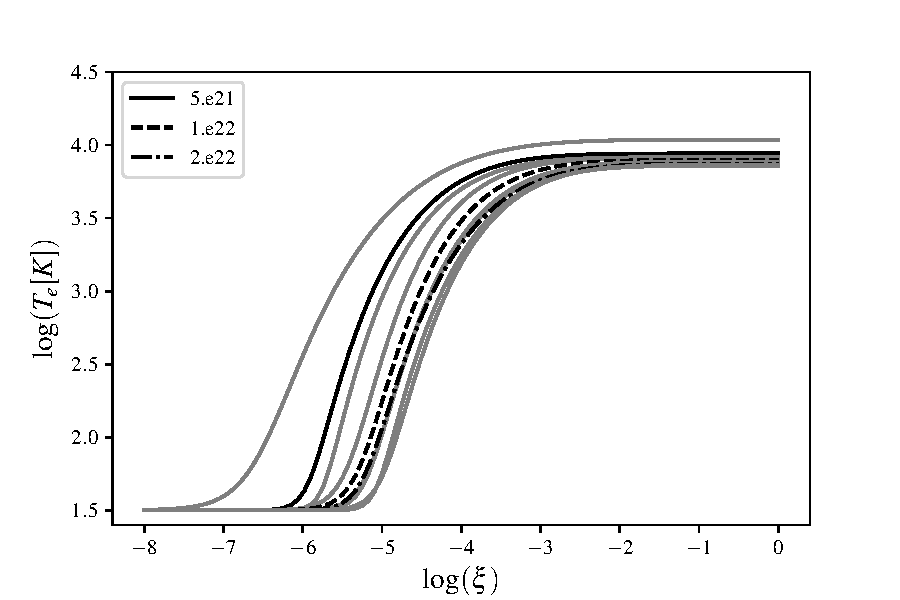
\includegraphics[width=.45\textwidth]{Fig1}
    \caption{Temperature as a function of the ionization parameter, where $3$ selected column densities are highlighted. \label{fig:tempxi}}
\end{figure}

The dust temperatures and initial density structure are calculated using the D’Alessio
Irradiated Accretion Disk (\textsc{DIAD}) radiative transfer models \citepads{1998ApJ...500..411D,1999ApJ...527..893D,2001ApJ...553..321D,2005ApJ...621..461D,2006ApJ...638..314D}, that best fit the median spectral energy distribution (SED) in Taurus.
The gas temperatures are assumed to be completely coupled to the dust temperature for $N>N_X$.

\begin{table*}
\caption{Star and disc properties}
\label{tab:stars}
\centering
\begin{tabular}{c c c c c c c c c}
\hline
$M_\star$ [$M_\odot$] & $R_\star$ [$R_\odot$] & ST & $L_\star$ [$L_\odot$] & $L_X$ [$10^{29}$ erg/s] & $T_\star$ [K] & M$_\mathrm{d}$ [$M_\odot$] & R$_{in}$ [au] & R [cells]\\
\hline
\hline
   $1.0$ & $2.615$ & K6 & $2.335$ & $20.4$ & $4278$ & $0.0444$ & $0.445$ & $412$\\
   $0.5$ & $2.125$ & M1 & $0.9288$ & $7.02$ & $3771$ & $0.0363$ & $0.2225$ & $449$\\
   $0.3$ & $2.310$ & M5 & $0.6887$ & $3.20$ & $3360$ & $0.0292$ & $0.1335$ & $477$\\
   $0.1$ & $1.055$ & M6 & $0.08559$ & $0.589$ & $2928$ & $0.0264$ & $0.0445$ & $535$\\
\hline
\end{tabular}
\end{table*}

\subsection{Hydrodynamical model}\label{sec:hydro-model}

We performed a set of hydrodynamical simulations using the \textsc{PLUTO} code \citepads{2007ApJS..170..228M}, adopting a spherical coordinate system centred on to the star.
The grid is logarithmically spaced in the radial direction, in order to have better resolution in the inner region of the disc, where photo-evaporation is mostly effective.
At the same time, it allows us to model the disc out to large radii ($R_{out}= 1000$ au) without increasing strongly our computational costs and preventing boundary effects that can affect the stability of the wind flow.
For a detailed discussion of the numerical artifacts induced by the grid outer boundary, the reader is referred to \citetads{2019MNRAS.487..691P}.
The grid is spaced linearly in the polar direction to maximize the resolution at the wind launching region.

We initially evolve the system for $100$ orbits at \si{10}{au} without stellar irradiation, in order to reach a quasi-hydrostatic equilibrium.
Then, we switch on the stellar heating (applied through a parameterisation from the radiative transfer simulation, as explained in Sec.~\ref{sec:thermal-calc} and \citetads{2019MNRAS.487..691P}) and continue to evolve the system until the cumulative mass-loss rate and gas streamline in the wind have reached a stable configuration.

%-------------------------------------------------------------------
\section{Results}\label{sec:results}
%-------------------------------------------------------------------

\subsection{Mass-loss rates}\label{sec:mdot}
We integrated the gas flow along the streamlines during the last 200 orbits of each simulation and plotted the resulting cumulative mass-loss rates as a function of stellar masses in a sqaure-box plot in Fig.~\ref{fig:Mdot}, where we included also the run with a $0.7$ $M_\odot$ star from \citetads{2019MNRAS.487..691P}, which has been rescaled in order to have the same stellar mass--X-ray luminosity adopted in these runs following eq.~\ref{eq:Lx}.
\begin{figure}
  \centering
  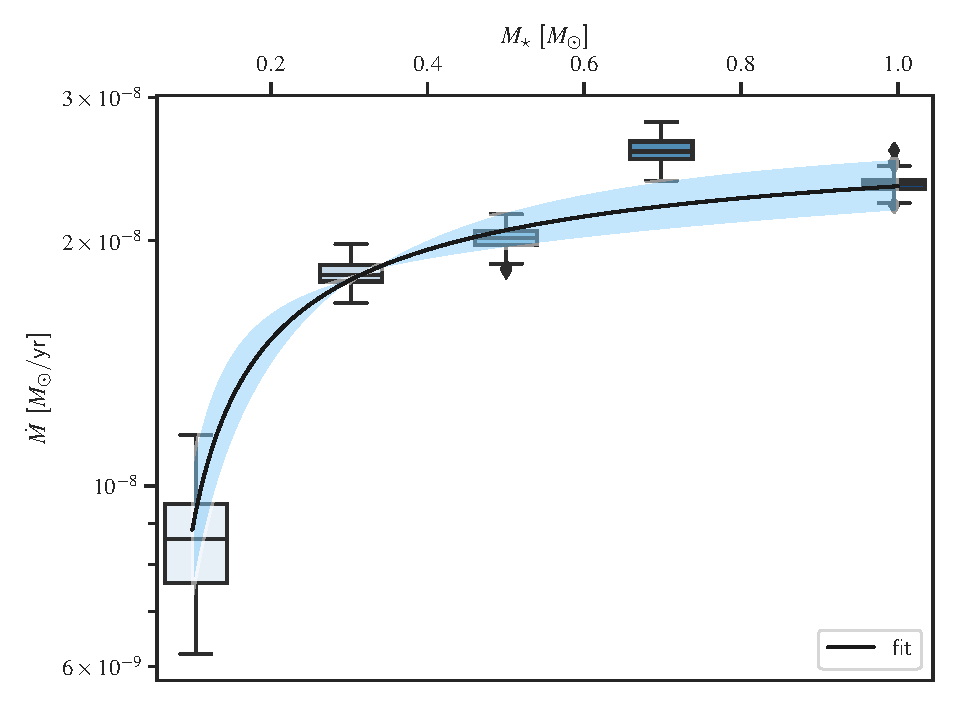
\includegraphics[width=0.45\textwidth]{mdot}
  \caption{Cumulative mass-loss rate as a function of stellar mass. \label{fig:Mdot}}
\end{figure}
A fitting function has been overplotted with a solid line, which shows the steeper dependance of the mass-loss rate for the lower end of stellar mass studied, while it becomes much flatter around few times $10^{-8}$ for $M_\star > 0.3 M_\odot$.
This behavior is in contrast with the much shallower dependance on the stellar mass derived in \citetads{2012MNRAS.422.1880O}. In Appendix~\ref{sec:owen} we compare the two profiles.
The reason for the discrepancies are the difference in the disc structure, due to the variation of stellar mass and bolometric luminosity (as calculated for a young stellar object by \citetads{2000A&A...358..593S}) that were not taken into account in \citetads{2012MNRAS.422.1880O}, the new prescription of the stellar temperature as a function of the column density that predicts higher mass-loss rates as shown already in \citetads{2019MNRAS.487..691P}, and the much more broader radial extent of the surface mass-loss rate profiles.
The best fitting function obtained from the current study is
\begin{equation}
  \dot{M} = 2.967\times10^{-8} - 6.325\times10^{-9} \left(\frac{M_\star}{M_\odot}\right)^{-0.518} [M_\odot\, \mathrm{yr}^{-1}]\,.
\end{equation}
In this analysis the dependance on the stellar X-ray luminosity is not considered, but the value adopted for the simulation is mass-dependant following \citetads{2007A&A...468..353G}
\begin{equation}\label{eq:Lx}
	\log_{10}{(L_X)} = (1.54 \pm 0.12) \log_{10}{(M_\star)} + (30.31 \pm 0.06)\,.
\end{equation}
We show in Figure~\ref{fig:Mdot} with a shaded light blue region the influence of the $1 \sigma$ error reporte in eq.~\ref{eq:Lx} on the cumulative mass-loss rate following the relation derived in \citetads{2019MNRAS.487..691P}
\begin{equation}\label{eq:MdotLx}
  \log_{10}(\dot{M}(L_X)) = A_\textrm{L} \exp{\left[\frac{(\ln{(\log_{10}(L_X))}-B_\textrm{L})^2}{C_\textrm{L}}\right]} + D_\textrm{L} [M_\odot\, \mathrm{yr}^{-1}]\,,
\end{equation}
with $A_\textrm{L} = -2.7326$, $B_\textrm{L} = 3.3307$, $C_\textrm{L} = -2.9868\cdot10^{-3}$, $D_\textrm{L} = -7.2580$.

\subsection{Wind profiles}\label{sec:wind-prof}
Deriving the integrated profile along the radial axis we obtain the radial distribution of the mass-loss rate shown in Figure~\ref{fig:Sigmadot}. The profiles look very similar regarding the maximum radial extent (up to ~200 au) and the mass-loss rate at intermediate radii (between 10 and 100 au). However, the change in the location of the maximum is affecting the resulting cumulative mass-loss rates, since the disc mass increases with radius.
\begin{figure}
  \centering
  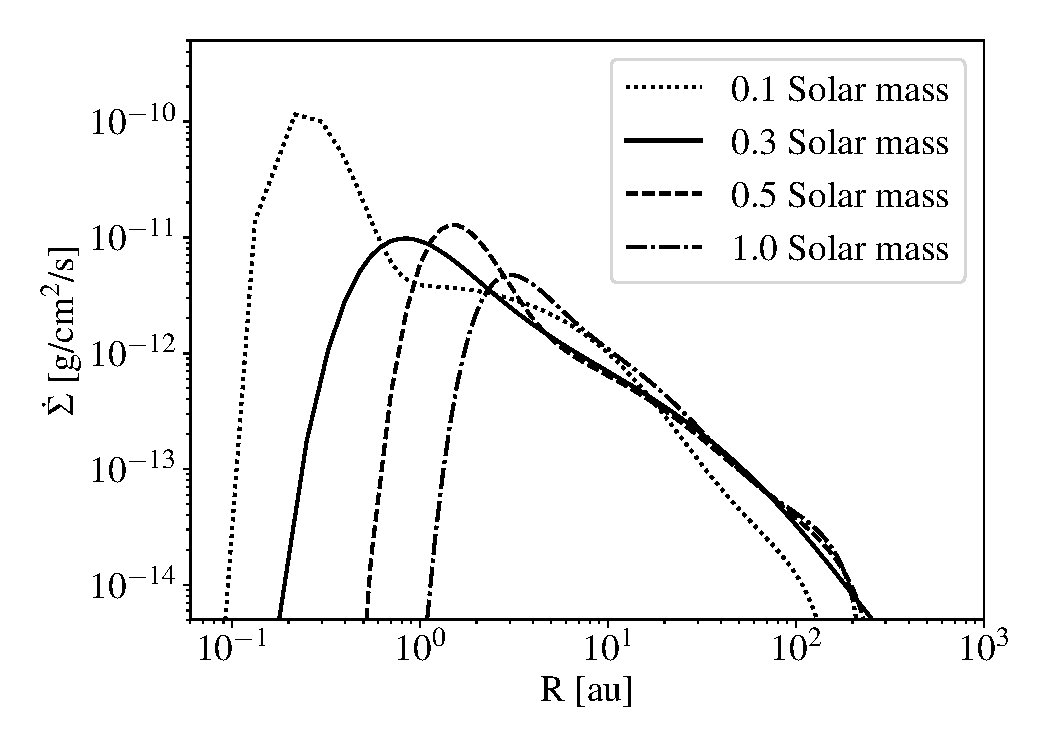
\includegraphics[width=0.45\textwidth]{Surfprofile}
  \caption{Surface density mass-loss rate profile for the different simulations. \label{fig:Sigmadot}}
\end{figure}
We then plotted in Figure~\ref{fig:maxProf} the location of the maxima of the different profiles. A stricking result is that the maxima are linearly increasing with stellar mass.
\begin{figure}
    \centering
    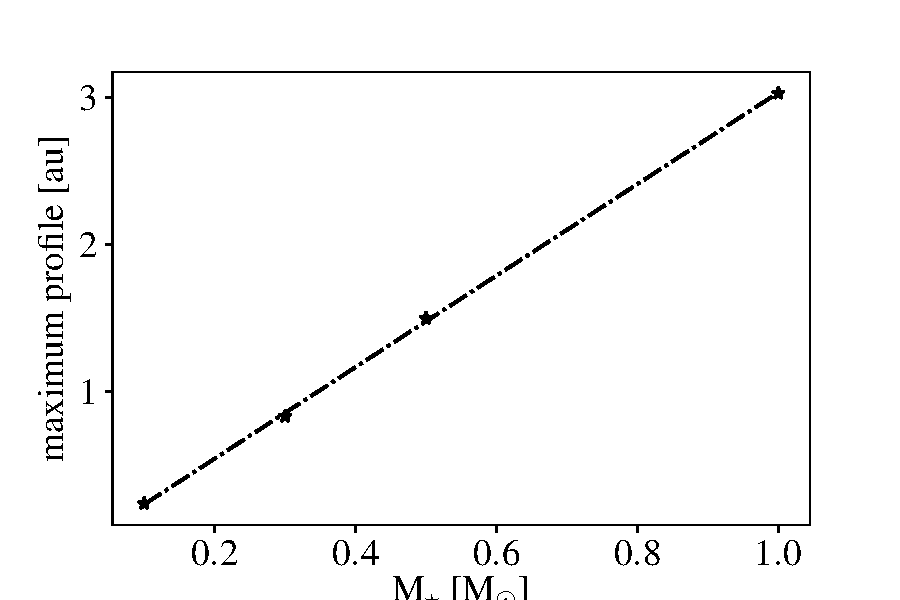
\includegraphics[width=0.45\textwidth]{maxProf}
    \caption{Maximum location of the surface density mass-loss rate profile for the different simulations. \label{fig:maxProf}}
\end{figure}
The characteristic physical scale to keep in mind in this context is the gravitational radius, which define the location where a gas parcel becomes unbound from the central star \citepads{1994ApJ...428..654H,2003PASA...20..337L}
\begin{equation}\label{eq:rg}
  r_g = \frac{\gamma-1}{2\gamma} \frac{GM_\star\mu m_H}{k_B T_0} \simeq 1.4 \left(\frac{T_0}{10^4 K}\right)^{-1} \left(\frac{M_\star}{1 M_\odot}\right) \ [au]\,,
\end{equation}
where $\gamma$ is the adiabatic index, $M_\star$ the stellar mass, $\mu$ the mean molecular weigth, $m_H$ the proton mass, $k_B$ the Boltzmann constant, and $T_0$ is the temperature at the base of the flow.
The maximum locations of the profiles should correspond with the locations of the effective gravitational radius. The fact that they are scaling linearly with stellar mass implies that the dependance on the gas temperature is not strong, and that the disc structure readjusts in order to have a similar temperature at the wind launching region for the different stellar (and disc) masses.
The best fitting function to the data is
\begin{equation}\label{eq:rg_sim}
  r_g = 3 \left(\frac{M_\star}{1 M_\odot}\right) \ [au]\,,
\end{equation}
which suggest that the temperature at the base of the flow at the gravitational radius is about $T_0 \simeq 5000 K$.
The best fit for the surface mass-loss rate is given by the following function, as in \citetads{2019MNRAS.487..691P}
\begin{eqnarray}
  \dot{\Sigma}_w(R) &= \ln{(10)} \bigg(\frac{6\, a\, \ln{(R)}^5}{R\, \ln{(10)}^6} +
  \frac{5\, b\, \ln{(R)}^4}{R\, \ln{(10)}^5} +
  \frac{4\, c\, \ln{(R)}^3}{R\, \ln{(10)}^4} + \\ \nonumber
  &\frac{3\, d\, \ln{(R)}^2}{R\, \ln{(10)}^3} +
  \frac{2\, e\, \ln{(R)}}{R\, \ln{(10)}^2} + \\ \nonumber
  &\frac{f}{R\, \ln{(10)}}\bigg)
  \frac{\dot{M}_w(R)}{2\pi\, R} \ [M_\odot\, {au}^{-2}\, {yr}^{-1}]\,
\end{eqnarray}
with
\begin{equation}
  \dot{M}_w(R) = \dot{M}(L_X) 10^{a\log{R}^6 + b\log{R}^5 + c\log{R}^4 + d\log{R}^3 + e\log{R}^2 + f\log{R} + g}\,
\end{equation}
where the parameters for the different stellar masses are given in Table~\ref{tab:fit}
\begin{table*}
\caption{Parameters for the Surface density profiles}
\label{tab:fit}
\centering
\begin{tabular}{c c c c c c c c c}
\hline
$M_\star$ [$M_\odot$] & a & b & c & d & e & f & g & $\dot{M}$ [$10^{-8}$ $M_\odot$ \ yr]\\
\hline
\hline
   $1.0$ & $-0.6744$ & $6.0115$ & $-21.7353$ & $40.8882$ & $-42.6090$ & $24.5487$ & $-7.4008$ & $2.3519$\\
   $0.5$ & $-0.2894$ & $2.5582$ & $-9.0723$ & $16.3130$ & $-15.4514$ & $7.9860$ & $-3.0702$ & $2.0162$\\
   $0.3$ & $-0.0320$ & $0.3563$ & $-1.5210$ & $3.0815$ & $-3.1463$ & $2.5411$ & $-2.3672$ & $1.8199$\\
   $0.1$ & $-0.1656$ & $1.0352$ & $-2.1617$ & $1.3152$ & $0.5770$ & $0.3949$ & $-1.5815$ & $0.8801$\\
\hline
\end{tabular}
\end{table*}

\subsection{Disc structure and gas streamlines}\label{sec:streamlines}
The topology of the gas streamlines is strongly dependent on the underlying disc structure. This behavior has already been studied in the context of transitional discs \citepads[see e.g.][]{2019MNRAS.487..691P}, where at the inner edge of the disc the gas streamlines are moving inwards before curving and leave the disc radially.
In Figure~\ref{fig:streamlines} we show the gas streamlines for the $0.1 M_\star$ for which this effect is stronger. There is a change in the direction of the streamline curvature at the base of the flow corresponding to a change in the sign of the disc aspect ratio gradient, as shown in Figure~\ref{fig:hr}.
While for $r<r_g\sim 0.3$ au the gas is still gravitationally bound, the stellar irradiation can move it to larger radii where it can leave the system. As a result, inside $0.3$ au the gas is moving outwards, while outside it is accelerating moving inwards before leaving radially the disc, creating around $0.3$ au a maximum in the profile for the surface mass-loss rate.
\begin{figure}
    \centering
    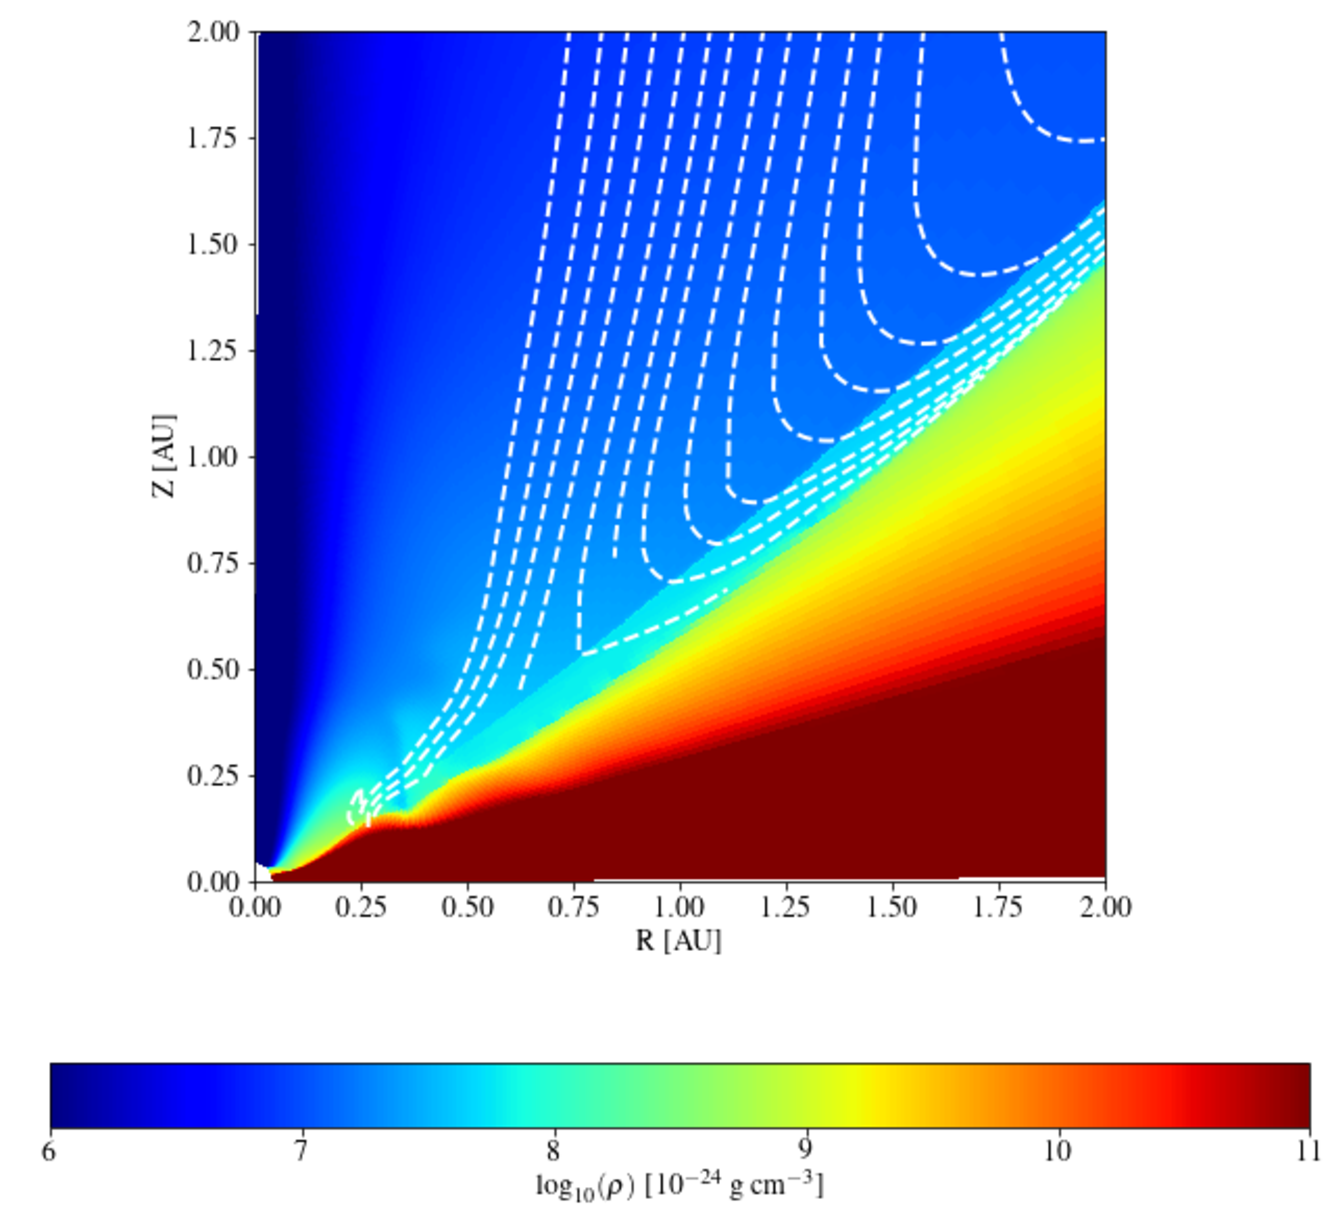
\includegraphics[width=0.45\textwidth]{streamlines}
    \caption{Density distribution in the inner 2 au of the run with a 0.1 $M_\odot$ where the gas streamlines every $1\%$ of the cumulative mass-loss rate are overplotted. \label{fig:streamlines}}
\end{figure}
This effect is much stronger for low stellar luminosities, as highlighted in the inset of Figure~\ref{fig:hr}.
\begin{figure}
    \centering
    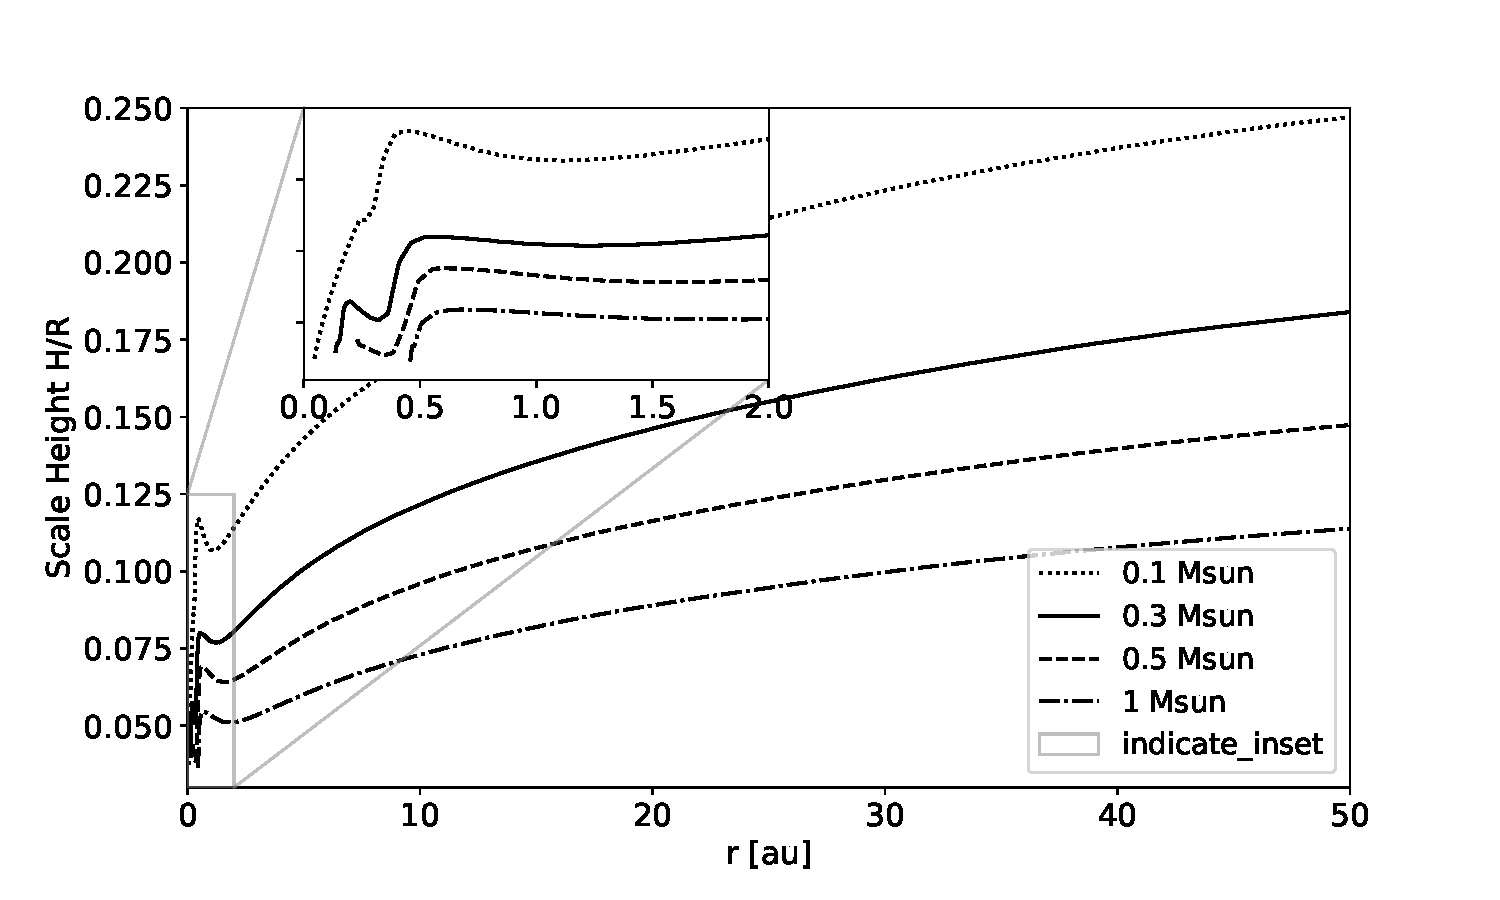
\includegraphics[width=0.45\textwidth]{HR_comp}
    \caption{Disc aspect ratio in the inner 50 au of the different runs perfomed. In the inset a zoom in on the inner 2 au is shown to highlight the change in the sign of the aspect ratio gradient which is related to a change in the topology of the streamlines at the base of the flow. \label{fig:hr}}
\end{figure}
The final disc density distribution for the different stellar masses (and luminosities) is shown in Figure~\ref{fig:discs} where the strong increase in the disc aspect ratio as a function of stellar mass is highlighted.
\begin{figure*}
    \centering
    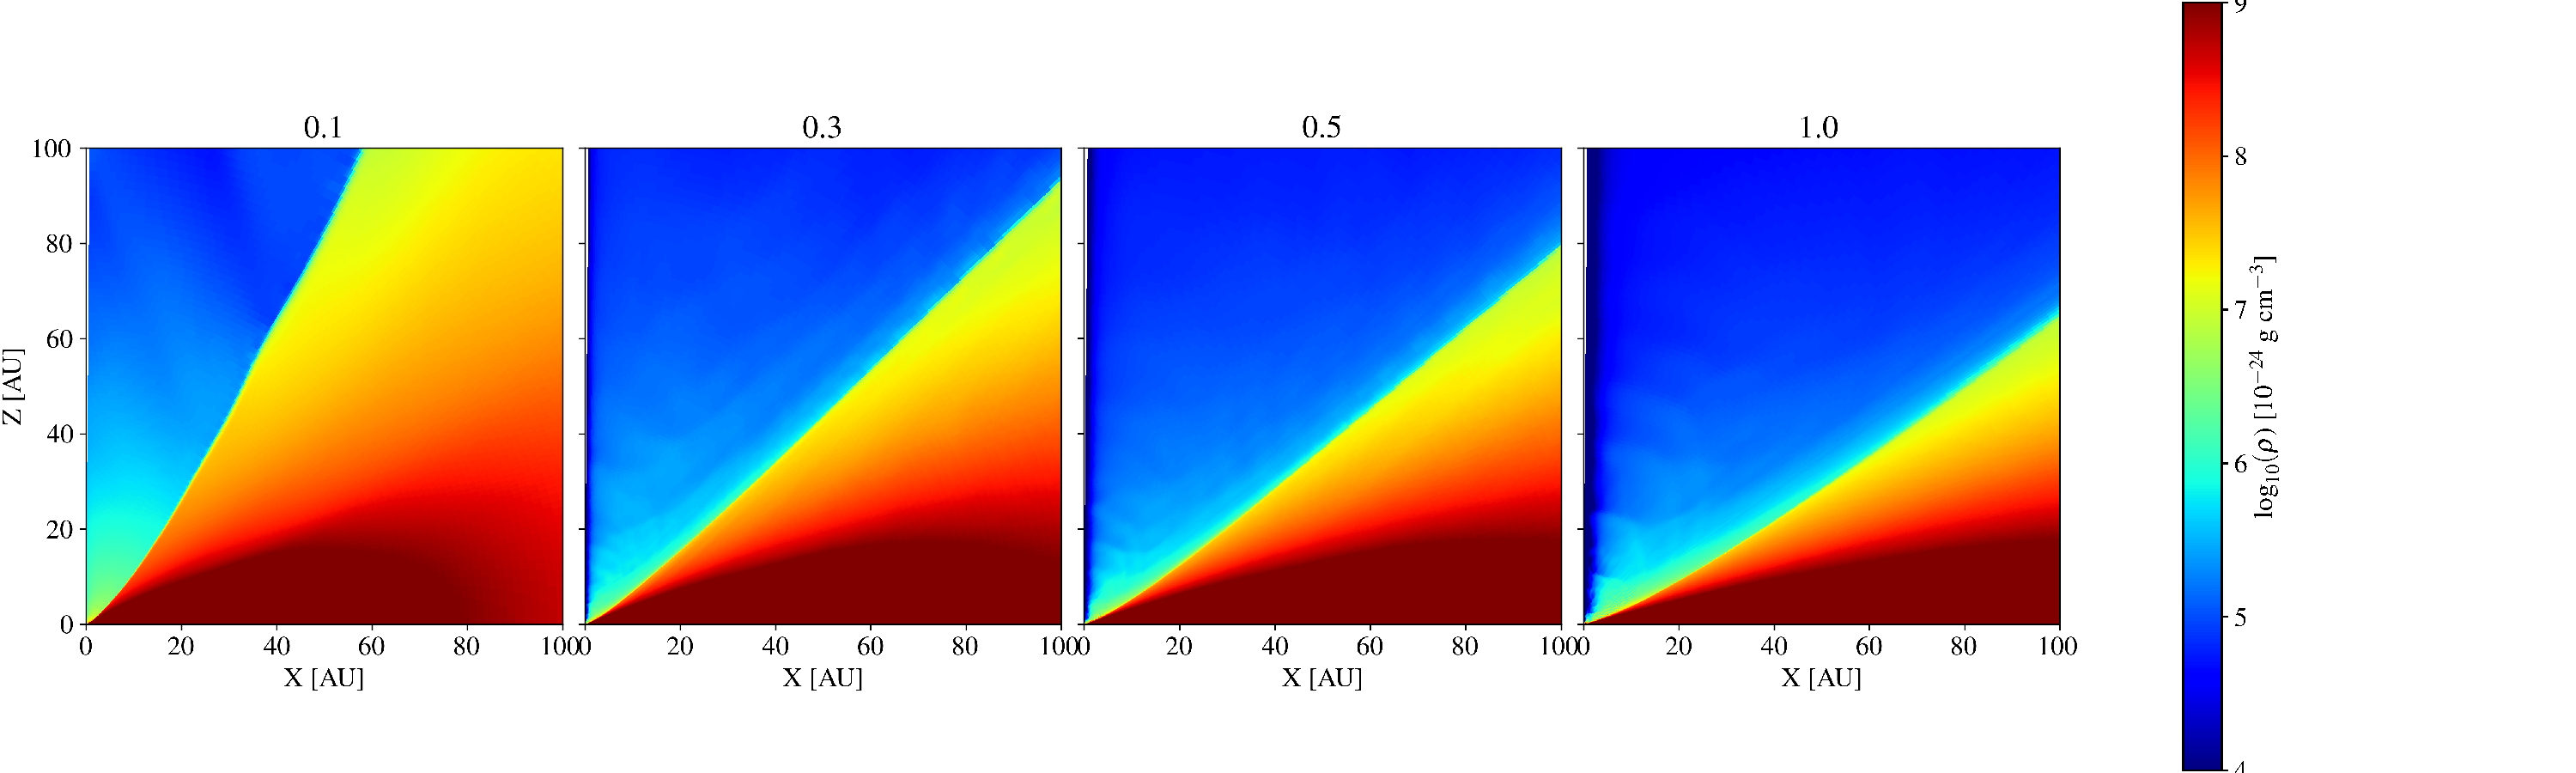
\includegraphics[width=\textwidth]{disc}
    \caption{Density distribution in the inner 100 au for the the differen runs. \label{fig:discs}}
\end{figure*}
The larger flare in the disc structure for low stellar masses compensates the lower penetration depth of the high energetic X-ray irradiation, producing only a modest difference in the final cumulative mass-loss rate.

The self-similarity of gas streamlines across different stellar masses proposed by
\citetads{2012MNRAS.422.1880O} is then lost both close to the disc surface because of the different curvature of the streamlines, and also at larger radii due to the increase of the disc aspect ratio as a function of stellar mass and luminosity.

%\subsection{Sonic surface}\label{sec:sonic-surface}
%The analysis of \citetads{2012MNRAS.422.1880O} is based on the assumption that the properties of the mass-flux can be determined at the sonic surface, and that the sound speed is roughly given by the Parker value
%\begin{equation}
%  c_s^2 = \frac{GM_\star}{2R}
%\end{equation}
%An important assumption is that the height of the sonic surface is not much larger than its cylindrical radius ($z_s \ngg R$), which can brake down for lower stellar masses, since the disc flaring is proportional to the central mass.

%-------------------------------------------------------------------
\section{Conclusions}\label{sec:conclusions}
%-------------------------------------------------------------------

  We expanded the study of \citetads{2019MNRAS.487..691P} of the mass-loss rate profiles due to XEUV irradiation from the central star probing different stellar masses.
  We found that

   \begin{enumerate}
      \item stellar irradiation has a strong impact on the underlying disc structure, increasing the disc aspect ratio and causing a large flaring for low X-ray luminosities (see Figs.~\ref{fig:hr},\ref{fig:discs})
      \item the large disc flaring is changing the streamline topology close to the wind launching region for the 0.1 $M_\odot$, generating an accelerating flow moving outwards inside the gravitational radius, and moving inwards outside of it (see Fig.~\ref{fig:streamlines})
      \item we provide fitting function for the surface mass-loss rate profiles for different stellar masses whose luminosity is scaled based on eq.~\ref{eq:Lx}.
      \item the maximum of the mass-loss profiles, which corresponds to an effective gravitational radius, is independent of the temperature at the base of the flow, since the disc is readjusting based on the stellar X-ray luminosity, and it is given by $r_g=3M_\star$
      \item the resulting cumulative mass loss rate scales as $M_\star^{-0.518}$, with a profile which is much steeper than the one derived in \citep{2012MNRAS.422.1880O}. The discrepancy is coming from having an improved temperature prescription as a function of column density which, together with the larger disc aspect ratio as a function of stellar mass, gives a much radially extended photoevaporation profile.
   \end{enumerate}

\begin{acknowledgements}
    GP acknowledges support from the DFG Research Unit ‘Transition Disks’ (FOR 2634/1, ER 685/8-1).
    This work was performed on the computing facilities of the Computational Center for Particle and Astrophysics (C2PAP).
\end{acknowledgements}

\begin{appendix}
\section{Comparison with Owen 2012}\label{sec:owen}
The result of this work predicts consistenly larger mass-loss rates with respect to the previous analysis by \citetads{2012MNRAS.422.1880O}.
\begin{figure}
  \centering
  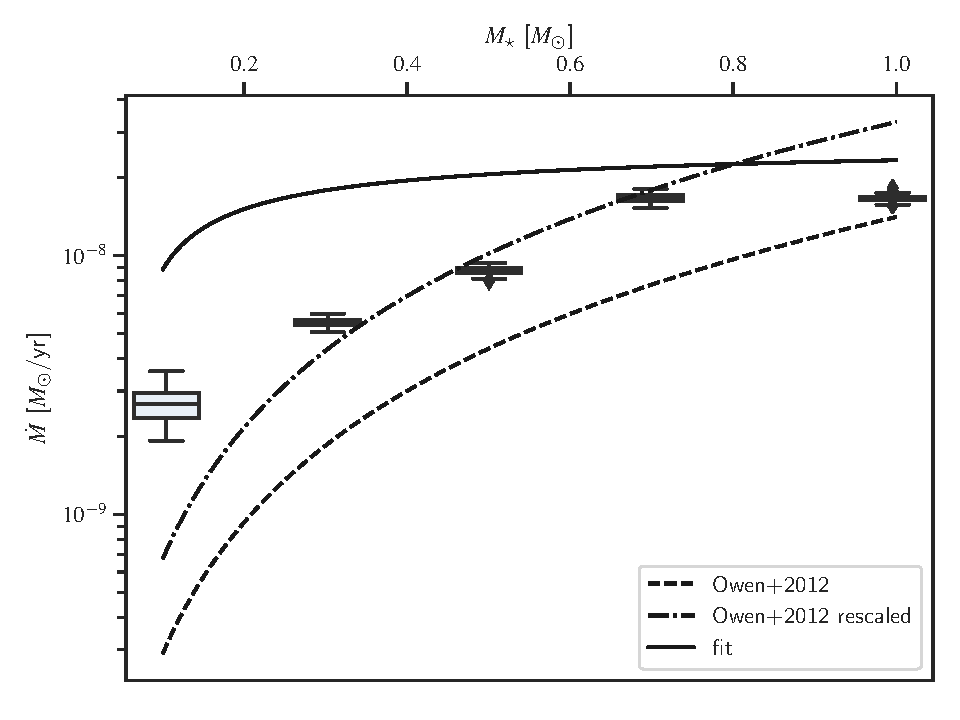
\includegraphics[width=.5\textwidth]{mdot_comp}
  \caption{Cumulative mass-loss rate as a function of stellar mass scaled to reproduce the same disc extent as in \citetads{2012MNRAS.422.1880O}. The profile from \citetads{2012MNRAS.422.1880O} is overplotted with a dashed line, and its scaled version to fit the 0.7 $M_\odot$. \label{fig:mdot_comp}}
\end{figure}
One of the main difference in the profiles obtained in the current work is its radial extent. \citetads{2012MNRAS.422.1880O} performed 2 simulations for a $0.1$ and $0.7$ $M_\odot$ from which they derived a scaling law for the outer edge of the profiles as an exponential cut.
When we apply the same cut in the radial extent of our profiles, as shown in Figure~\ref{fig:mdot_comp}, we obtain values much closer to the one derived in their study. Furthermore, we scale their relation to fit the value of the $0.7$ $M_\odot$ showing that the resulting relation is fairly able to reproduce our current results.
The results of these 2 different studies can then be related when the different radial extent of the profiles, and the different temperature prescription are taken into account.

\section{Variation of stellar mass at constant}

\end{appendix}

\bibliographystyle{aa}
\bibliography{biblio}{}

\end{document}
